
% !TEX program = pdflatex
% !TEX enableSynctex = true
% !BIB program = bibtex


\documentclass[12pt]{article}

\usepackage{setspace}
\usepackage{amsmath}
\usepackage{amsfonts}
\usepackage{graphicx}
\usepackage{float}
\addtolength{\oddsidemargin}{-.7in}
\addtolength{\evensidemargin}{-.7in}
\addtolength{\textwidth}{1.4in}
\usepackage{enumerate}
\onehalfspacing
\usepackage{geometry} % Required for customizing page layout

\usepackage{caption}
\usepackage{booktabs}

\usepackage{hyperref}
\hypersetup{
	pdfstartview = FitH,
	pdfauthor = {...},
	pdftitle = {...},
	pdfkeywords = {...; ...; ...; ...},
	colorlinks = true,
	linkcolor = blue,
	urlcolor = blue,
	citecolor = blue,
	linktocpage=true
}


\DeclareMathOperator{\E}{\mathbb{E}}
\DeclareMathOperator*{\argmax}{arg\,max}
\DeclareMathOperator*{\argmin}{arg\,min}

\begin{document}
\section*{Partial equilibrium model - firms' problem}
\subsection*{Ver 1 - PE model - Fixed q-s - 3 state variables}
Productivity process: two-state markov chain \vspace{3mm} \\
Labour policy: 
\begin{equation}
    n(k,\varepsilon_i) = \left( \dfrac{ \nu \varepsilon_i k^\alpha}{w} \right)^{\frac{1}{1-\nu}}
\end{equation}
Corresponding output: 
\begin{equation}
    y(k,\varepsilon_i) = \varepsilon_i k^{\alpha} \left( \dfrac{\nu \varepsilon_i k^\alpha}{w} \right)^{\frac{\nu}{1-\nu}}
\end{equation}
Corresponding profits: 
\begin{equation}
    \pi(k,\varepsilon_i) = (1-\nu) y(k,\varepsilon_i) - c
\end{equation}
External finance premium - just a parameter \vspace{2mm} \\
Value function:
\begin{equation}
     V(k,b, \varepsilon_i) = \max_{k',b'}  \left( \pi(k,\varepsilon_j)+(1-\delta)k - k' +  q^s b' -b  +
            \beta (1-P_\chi) \sum_{j=1}^{N_\varepsilon} g_{ij}  V(x',\varepsilon_j') \right)
\end{equation}
\noindent Here, the firm can directly choose $k'$ and $b'$, which makes coding the transition matrix easier, since you do not have to interpolate the Q-es. In the end you just have some very sparse matrices, since the model is almost deterministic. \vspace{3mm} \\
The shortcoming is you have 3 state variables and 2 action variables, which means that it is very hard to move past a grid size of 30. 

\newpage
\setcounter{equation}{0}


\subsection*{Ver 2 - Fixed Qs - cash on hand - two-state productivity}
Productivity process: two-state markov chain \vspace{3mm} \\
Labour policy: 
\begin{equation}
    n(k,\varepsilon_i) = \left( \dfrac{ \nu \varepsilon_i k^\alpha}{w} \right)^{\frac{1}{1-\nu}}
\end{equation}
Corresponding output: 
\begin{equation}
    y(k,\varepsilon_i) = \varepsilon_i k^{\alpha} \left( \dfrac{\nu \varepsilon_i k^\alpha}{w} \right)^{\frac{\nu}{1-\nu}}
\end{equation}
Corresponding profits: 
\begin{equation}
    \pi(k,\varepsilon_i) = (1-\nu) y(k,\varepsilon_i) - c
\end{equation}
Future cash on hand: 
\begin{equation}
   x' = \pi(k',\varepsilon_j')+(1-\delta)k'-b'
\end{equation}
External finance premium 
\begin{equation}
    q^s = 0.94
\end{equation}
Need an equity finance option. Otherwise there certain states are not associated to any feasible action. Here, I assume. This means that firms will sometimes have negative cash on hand. 
\begin{equation}
    d < 0 \implies d = 1.6d
\end{equation}
Value function:
\begin{equation}
     V(x,\varepsilon_i) = \max_{k',b'}  \left(x - k' +  q^s b' + 
            \beta  (1-P_\chi)  \sum_{j=1}^{N_\varepsilon} g_{ij} V(x',\varepsilon_j') \right)
\end{equation}
Adding cash on hand reduces the grid to 2 state and 2 action variables. This implies that you can do a much larger grid. However, you have to interpolate resulting x that follows from choices k' and b' to the grid, since x-here is the result. This could be a problem. Generally, results are well behaved in this case, although they are very mechanical. 


\begin{figure}[H]  % [h] indicates placing the image here
    \centering
    \caption{Ver2 - prod: 5, 8} \label{chart:CFLcdf}
    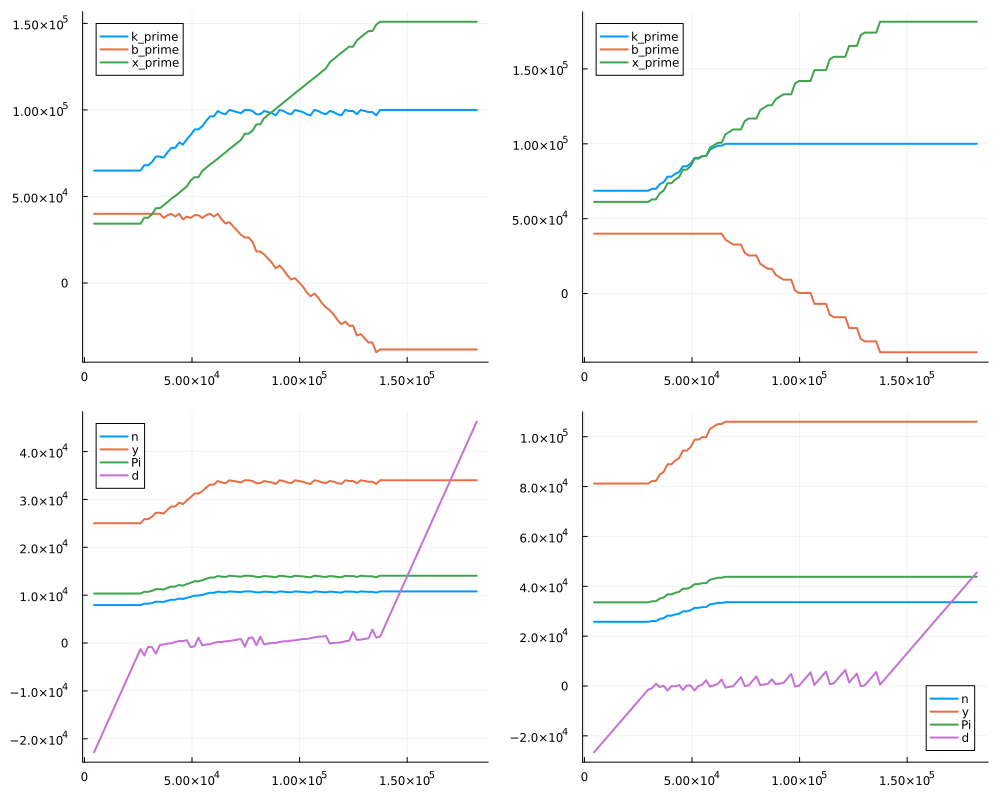
\includegraphics[width=1\textwidth]{ver2.png}
\end{figure}


\newpage
\setcounter{equation}{0}

\subsection*{Ver 3 - ABL Qs - cash on hand - AR(1) productivity}
Productivity process: AR(1) process with multiple states. Below, I plot the worst the median and the best productivity state. \vspace{3mm} \\
Labour policy: 
\begin{equation}
    n(k,\varepsilon_i) = \left( \dfrac{ \nu \varepsilon_i k^\alpha}{w} \right)^{\frac{1}{1-\nu}}
\end{equation}
Corresponding output: 
\begin{equation}
    y(k,\varepsilon_i) = \varepsilon_i k^{\alpha} \left( \dfrac{\nu \varepsilon_i k^\alpha}{w} \right)^{\frac{\nu}{1-\nu}}
\end{equation}
Corresponding profits: 
\begin{equation}
    \pi(k,\varepsilon_i) = (1-\nu) y(k,\varepsilon_i) - c
\end{equation}
Future cash on hand: 
\begin{equation}
   x' = \pi(k',\varepsilon_j')+(1-\delta)k'-b'
\end{equation}
External finance premium:
\begin{equation}
    q^{abl}(k',b')b' = \beta \left[ (1-P_\chi) b' + P_\chi \min\{b', \ \phi_k (1-\delta) k' \} \right]  
\end{equation}
Equity finance option:
\begin{equation}
    d < 0 \implies d = 1.6d
\end{equation}
Value function:
\begin{equation}
     V(x, \varepsilon_i) = \max_{k',b'}  \left( x - k' +  q(k',b',\varepsilon) b' +
            \beta (1-P_\chi) \sum_{j=1}^{N_\varepsilon} g_{ij}  V(x',\varepsilon_j') \right)
\end{equation}
Here the two innovations are that interest rates are endogenous and the productivity process is more realistic. Results makes sense, although they display this jigsaw pattern in certain regions and calibrations. \textbf{Weirdly, the model breaks down when grids are defined logarithmically.} Firms very quickly converge to their desired level of capital, even if they are cash-poor - that is because $q$ remains relatively large even for very indebted firms.

\begin{figure}[H]  % [h] indicates placing the image here
    \centering
    \caption{Ver3 - worst, median and best productivity states} \label{chart:CFLcdf}
    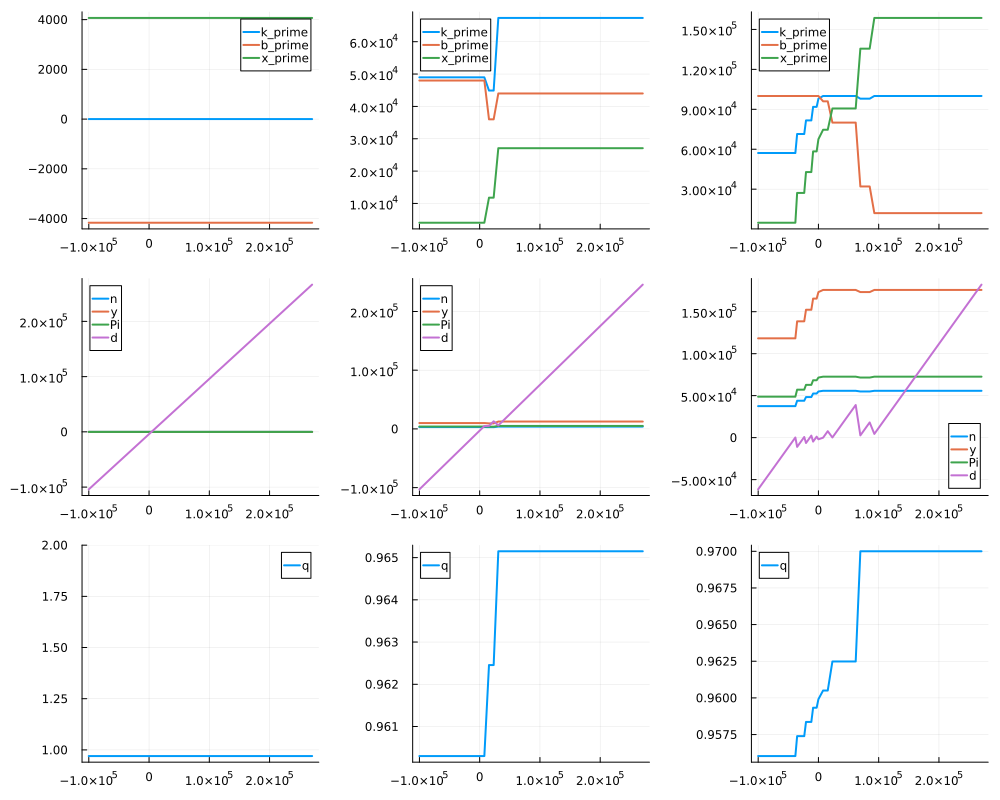
\includegraphics[width=1\textwidth]{ver3.png}
\end{figure}

\newpage
\setcounter{equation}{0}

\subsection*{Ver 4.1 - Endogenous defaults, and better x-interpolation}
\textbf{Same as in Ver 3:} AR(1) productivity process, Labour policy; Corresponding output; Corresponding profits; Future cash on hand; External finance premium. \vspace{3mm} \\
Equity finance option is not necessary anymore, but I keep it with prohibitive costs. This is needed to ensure that firms have a feasible action every state.  \vspace{3mm} \\
Default decision: the firm chooses $\sigma(x, \varepsilon)$ and the corresponding $V(x, \varepsilon)$. It chooses default if $V(x,\varepsilon) \leq 0$ and $x \leq 0$ - hence the firm can fall back to limited liability and the associated value is zero. \vspace{3mm} \\
Exit decision (not implemented in this version): the firm can decide to quit without falling back to limited liability. The associated value is the cash on hand: $x$. The firm chooses this if $V(x, \varepsilon) \leq x$ and $x \geq 0$. \vspace{3mm} \\
Value functions:
\begin{equation}
    V_0 = \max \{ V_{def}, V_{exit}, V_{cont} \}
\end{equation}
where $ V_{def} = 0$, $V_{exit} = x$ and $V_{cont}$ is
\begin{equation}
     V_{cont}(x, \varepsilon_i) = \max_{k',b'}  \left( x - k' +  q(k',b',\varepsilon) b' +
            \beta (1-P_\chi) \sum_{j=1}^{N_\varepsilon} g_{ij}  V_0(x',\varepsilon_j') \right)
\end{equation}
When a firm chooses $(k',b')$ it can expect a realization of $x$, given its current $\varepsilon$. The problem is that this may not lie on the $x$ grid. In previous versions, I chose the $x_i$ on the grid that was closest to the realization of $x$. This has led to some imprecisions. Here, I make the following adjustment: if observe the two gridpoints that surround the realization of $x$. These are defined as $x_{low}$ and $x_{high}$. \vspace{3mm} \\
Then, assume that the probability of falling on these points linearly depends on the relative distance $x_{low}$ and $x_{high}$. This yields more stable results, but computing the optimal policies becomes much slower. It is probably because the Q matrix becomes more dense when with adjustment. Also, setting up Q takes longer.

\subsection*{Ver 5 - default probabilities and endogenous interest rates}

In previous iterations of the model, the interest rate was calculated on the basis of an exogenous default probability. Now you have a default decision you can update the interest rates while taking into account the endogenous default probability. I follow the following algorithm: 
\begin{enumerate}
    \item Set $q|P_{d}(exo)$, the interest rate given the exogenous default probability. Then I calculate $V(x,\varepsilon)$ given $q|P_{d}(exo)$ - which allows me to calculate the default decision for each $(x,\varepsilon)$.
    \item Now it is possible to calculate what is the probability that the firm lands on a state $(x,e)$ associated with default. This corresponds to endogenous default probability $P_d(endo)|(x,e,k',b')$ - where $P_d(endo)$ is an $n \times m$ matrix containing the default probabilities for each state-action pair.
    \item Update interest rates taking into account the endogenous default probability $q|P_{d}(exo),P_{d}(endo)$ and recalculate the optimal $k',b$ and default policies
    \item Repeat $1-3$ until the optimal policies and interest rates do not change - that is, $ (k^{i},b^{i},\chi^{i},q^{i}) = (k^{i-1},b^{i-1},\chi^{i-1},q^{i-1}) $ for each state $(x,\varepsilon)$
\end{enumerate}
\textbf{Exit decision}: I also implement endogenous exit decision. This is analogous to the default decision, with the difference that firms may keep their cash on hand if they quit voluntarily. Moreover, you need to change the value of defaulting to some small negative value ($-1000$ in this calibration). Otherwise firms always prefer to just pay all cash on hand as dividends and stay on the market for one more period on the off chance that they receive a large, positive productivity shock. \vspace{3mm} \\
\textbf{Probability of default}: default can derive from an exogenous default shock or endogenous decision of the firm. The total probability of default can be described with:
$$             P_D = 1 - [(1 - P_{exo})(1 - P_{endo})]   $$ 
I will use this formula in the following.
\newpage

\section*{Summary of models up to Ver 5}

\textbf{Measure of size problem}: The cash on hand approach does not have a good measure of current size. The current cash on hand might be misleading since large debt might cancel out large capital stocks. You could do next periods' expected cash on hand, or next period's capital stock. \vspace{3mm} \\
\textbf{On interest rates}: You can rarely see default probabilities over 4\%. This does not mean that financial frictions are not significant. This is because the probability of default jumps at some point at a certain debt policy. This implies very high interest rates, which is not a good deal for the firm. Therefore in most cases, firms stop short of high levels of debt that would increase their default probabilities too much. \vspace{3mm} \\
\textbf{On debt debt policy of firms}: Here firms discount future by $\beta(1-P_\chi)$, whereas the fully secured interest rate is $\beta$. Therefore, when the firms manages to be fully secured, it prefers to hold a lot of debt and pay higher dividends, because if it defaults next period it might have to fall back on limited liability. This implies that even large, cash rich companies hold a lot of debt. Not a bad result, but probably not for the right reasons. \vspace{3mm} \\
\textbf{Firm growth}: Firms grow very quickly to their efficient sizes. A firm with no cash on hand has easy access to a lot of debt, and can grow out of cash-poorness very quickly. This might be a problem when I want to focus low wealth but productive firms. Try the reparametrization of the model - although gains here will probably be limited. Also you can also try adding a fixed cost of liquidation (paid by the lender). The advantage of this is that it can be treated purely as a calibration parameter (as opposed to default probability and resale value of capital) \vspace{3mm} \\
\textbf{Conceptualizing negative cash on hand}. How would a firm enter with negative cash on hand? You can add entry costs (usually they are needed anyways). Also you can suppose that these are distributed in a way that firms with large and negative cash on hand may enter. This is needed if you want to have cash poor but productive firms in the model. 
\setcounter{equation}{0}

\subsection*{Ver 6 - Heterogeneous debt contracts}
\textbf{Same as in Ver 5:} AR(1) productivity process, Labour policy; Corresponding output; Corresponding profits; Future cash on hand; Default decision, Exit decision \vspace{3mm}  \\
Value functions:
\begin{equation}
    V_0 = \max \{ V_{def}, V_{exit}, V_{cont} \}
\end{equation}
where $ V_{def} = 0$, $V_{exit} = x$ and $V_{cont}$ is
\begin{equation}
     V_{cont}(x, \varepsilon_i) = \max_{k',b'}  \left( x - k' +  q(k',b',\varepsilon) b' +
            \beta (1-P_\chi) \sum_{j=1}^{N_\varepsilon} g_{ij}  V_0(x',\varepsilon_j') \right)
\end{equation}
External finance premium: 
\begin{equation} \label{eq:opt_tau}
    \begin{split}
        & q = \frac{\beta}{b'} \Big{[} (1-P_D)b' \ +  P_D \Big(\min \big\{ b', \ \  \gamma(k',b',\varepsilon) \left( (1-\tau') \phi_A (1-\delta) k' +\tau' \kappa \phi_A  (1-\delta) k' \right)  \\
        & \quad  +  \ (1-\gamma(k',b',\varepsilon))\left((1-\tau') \phi_A (1-\delta) k' +\tau' \left( \phi_C \E_{\varepsilon'|\varepsilon}V_2 (x', \varepsilon') - \zeta \right) \right) \big\} \Big) \Big{]} 
    \end{split}
\end{equation}
The firm has access to CF-based and asset-based debt contracts simultaneously. It chooses the optimal reliance on CF-backed debt, $\tau$ to maximize $q$. Therefore, the $\argmax$ of equation 3 describes optimal CFL reliance. The solution strategy is the same as in version 5, but now it is much more complex, hence it is also more prone to error.
\begin{enumerate}
    \item Set $q^0$, the starting interest rate at $\beta$ and calculate the value of the firm, $V(x,\varepsilon)$ and $k', b'$ and exit policies given  $q^0$. 
    \item Calculate the following: the probability of default $P_D$, the probability of liquidation under default $\gamma$, the liquidation value; $\phi_A (1-\delta) k'$ and the reorganization value; $V_2 (x', \varepsilon') - \zeta$ given $q^0$, for each state-action pair - meaning that all these are $n \times m$ matrices.
    \item Update interest rate, $q^1$ associated with the state-action pair, taking into account the default and liquidation probability and lenders in-default payoffs. To do this, you also need find $\tau^1$ what maximizes $q^1$ for each state-action pair. This requires an additional loop, that calculates $q^1$ given tau, and then chooses the best $\tau$.
    \item Repeat $1-3$ until the optimal policies and interest rates do not change - that is, $ (k^{i},b^{i},\chi^{i},q^{i}) = (k^{i-1},b^{i-1},\chi^{i-1},q^{i-1}) $, or at least within some tolerance value for each state $(x,\varepsilon)$.
\end{enumerate}

\subsubsection*{Ver 6 - Problems and ideas}
\textbf{The linearity of q in CFL reliance:} \\
The expected in-default payoff of the lender after the asset-based debt is: 
$$  (1-\tau') \phi_A (1-\delta) k'  $$
for CF-based debt: 
$$    \tau'\left[\gamma(k',b',\varepsilon)(\kappa \phi_A  (1-\delta) k') +  (1-\gamma(k',b',\varepsilon))\left( \phi_C \E_{\varepsilon'|\varepsilon}V_2 (x', \varepsilon') - \zeta \right) \right] $$
The borrower chooses $\tau$ to maximize the sum of these two values. Since both of them depend on $\tau$ linearly, the optimal decision on $\tau$ is 0 if the first sum is larger and 1 of the second sum is larger. Hence, this setup still cannot reproduce CFL reliance in the range of $(0,1)$. The solution would be to add a $\gamma$ that increases in $\tau$. That is, higher reliance on CF based lending increases the chance of liquidation. This is realistic if the borrower can keep whatever is left after the default process and it gets to decide on liquidation. An example would be that a firms with a lot of unsecured debt chooses liquidation since lenders cannot enforce liquidation payments. this could deliver results, but it is not very realistic. \vspace{3mm} \\
\textbf{Adding extreme shocks}: with just the AR(1) productivity process, only a few firms end up close to cutoff values that yield non-extreme solutions. This could change if you added and extreme shock to productivity, which put firms into the best or the worst productivity bracket with some small probability.  \vspace{3mm} \\ 
\textbf{Issues of non-convergence}: sometimes this model version does not converge. There might be two reasons for this. First, it might be that the next $x$ with a particular debt decision falls closer to the non-default $x$ on the grid than the one associated with default. Then the lender offers the borrower a low interest rate even though the debt policy is not sustainable. In this case, the iteration is cut short. A quick solution is to increase the x-grid. A better one would be to do the same Xlow-Xhigh setup as in the Q matrix - \textbf{already implemented and it solves most convergence problems}. Second, the model practically converges, but there is oscillation between two neighboring debt levels and corresponding q-s. This can be solved with increasing the $b$ grid. Alternatively, you can just write a code that stops after this oscillation starts. Not very elegant but it is ok.

\newpage

\section*{General Notes}
\textbf{Taking logarithmic grids}: Results with logarithmic grids are not perfect, but they generally make sense. The problem is that some low cash on hand firms prefer to just produce a lot in the current period without accumulating assets - their production is financed by external finance almost entirely and their next period cash on hand is stuck at a low value. This is especially true for high productivity firms. This is not a bug (see the steadily increasing value in $x$) and it is not necessarily a problem, but it is a bit weird that firms of the same productivity do not converge to the same cash on hand - should check it under CFL borrowing. I should also add that this in every calibration, under some certain values very few firms actually do this. Making the discount parameter closer to one would probably solve this problem.   \vspace{3mm} \\
\textbf{Allowing for financial savings}:  Allowing $b$ to be negative means that a lot of firms with low productivity but high cash on hand do not exit immediately, but dismantles capital stock gradually. This would yield a gradual decline of financial wealth. Overall, results are nicer and converge faster, but of coarse the grid becomes less granular. With log grids and negative financial savings the model does not converge.  \vspace{3mm} \\
\textbf{Firm dynamics - Fmat fix} As its stands in earlier model version Fmat does not take into account exits in firm dynamics. This does not affect optimal firms choices (those are informed by Q and R) but it affects stationary distribution. Big masses of firms pile up in weird steady states that are associated with high liquidation probability. In later versions (up from ver7.2) this is fixed. Transition values in Fmat are scaled down with the endogeneous default probability, and a separate column for default-state is added. Overall the differences after the update are not large, but still visible. \vspace{3mm} \\
\textbf{The productivity process (Tauchen's method)}: \\
Productivity follows the AR(1) process:
$$ \ln(\varepsilon_{t+1}) = (1-\rho) \ln(\varepsilon_0) + \rho \ln(\varepsilon_t) + \sigma \zeta_\varepsilon $$
\begin{itemize}\setlength\itemsep{0em} \small
    \item $\rho$ is the persistence of the shock
    \item ln($\varepsilon_0$) is 'average productivity'm calibrated to $1$ in Kaas et al.
    \item $\sigma$ is the standard deviation of shocks
\end{itemize} \normalsize
I discretize the log-process via Tauchen's method, then take the exponents of the productivity values. This process does have some mean reversion in it, due to the first term on the RHS - however not every paper have this term, KT13 for instance does not. Moreover, I found two calibration approach: in Kaas, Öztürk and Kochen it is high persistence with $\rho$ close to one and small innovations whereas with KT13 and CandD, $\rho$ is around $2/3$ and innovations are large. In these papers there is no reversion to the mean in the AR process. Overall, I am not a hundred percent sure how to best set it.  \vspace{3mm} \\
\textbf{The determinants of firm size}: The Lukas type span of control parameter, and the price of the final good are the best to limit firm size. If you want more firms to participate (and firms participate from a lower cash on hand level) decrease the participation cost of entering.

\subsection*{Finding the stationary firm distribution}
Solution approach:
\begin{itemize} \setlength\itemsep{0em}
    \item Set up the VFI to find optimal policies given state variables and the wage, $w$ (some models solve for the price of the final good $p$, I use price as the numeraire so I can solve for the wage)
    \item Equilibrium wage is such that the value of entering is equal to the cost of entering: $V^e = k$ - this works only with entry decision 2. (see below)
    \item The stationary distribution is defined as follows in matrix form 
       $$ \mu = F(I-\text{diag}(X)) \mu + mf^0 = M\mu + mf^0 = m(I-M)^{-1}f^0 $$
       where $\mu$ is the distribution of firms, F is the transpose of the transition matrix given productivity shocks and policies; X denotes the exit policy; $f^0$ is the vector of entrants and $m$ scales the distribution of firms
    \item Defines the transition matrix of incumbents given production and exit policies and the productivity transition matrix $\rightarrow$ M
    \item Takes the vector of entrants $\rightarrow f^0$; in my model entrants may exit immediately, so $f_0$ should also be premultiplied with $I-\text{diag}(X)$
    \item The unscaled stationary distribution of firms ($\mu^{0}$) can be expressed as: 
        $$\mu^{0}= (I-M)^{-1}f^0$$
    \item Finds $m$ from labour market equilibrium given wage; 
        $N(w) = m \sum_\varepsilon \sum_x \mu^{0}_{x, \varepsilon} n_{x, \varepsilon} $
    \item Scales the stationary distribution $\mu = m\mu^0$ $\rightarrow$ $m$ is the measure of entrants but it scales the entire stationary distribution
\end{itemize}
 \textbf{On entry decision}: this must be figured out in order to have a stationary distribution of firms. In the Hopenhayn model the entry decision is made ex-ante, before learning about your productivity. Therefore, the value of entering is the same $V^e$ for each potential entrant. Under the free entry condition, $V^e = k$. I set up the model such that potential entrants first learn about their state and then decide to enter or not. This setup is designed to study composition of entrants under aggregate shock - as in Khan and Thomas. \vspace{3mm} \\
I see 3 ways:
\begin{enumerate} \setlength\itemsep{0em}
    \item Entrants decide in full knowledge of their ($x, \varepsilon$) - KT16, Kaas22
    \item Entrants decide ex-ante, knowing only $V^e$ - Hopenhayn, CandD
    \item Exogenous flow of entrants - Leo's recommendation, KT13, Öztürk (2023)
\end{enumerate}
Number 1 and 2 can be made almost equivalent setting the timing such that entrants do not produce in the current period. In this case, potential entrants uniformly face $V^e$. Then, they receive ($x, \varepsilon$) and can decide to exit, default or continue just as the rest of the incumbents. Hence, nonviable young firms exit after one period instead of not entering at the first place. The only difference to approach n1 is that it adds to the default and exit rates, but you can use the solution approach from above! \vspace{3mm} \\
Alternatively, you could have entry in the beginning of the period after which startups produce and decide to exit and or default. This is almost the same except that entrants take part in production. \vspace{3mm} \\
\textbf{Entrants' problem}: \\
There is a mass ($m$) of potential entrants that may enter after production has taken place. Entry decision is informed by the free entry condition, $\beta E[V^e(x,e)] - c_e = 0$ where $x_e$ the starting cash on hand and the $c_e$ is the setup cost. This decision takes effect at the end of the period, so firms quit without ever taking part in production. In this setting, entrants' problem is the same as incumbents', but their value is discounted by $\beta$ due to the timing. \vspace{3mm} \\
Define the joint starting distribution of $\Gamma(x,\varepsilon)$. Since $(x,\varepsilon)$ are independent in the beginning, you can just define the two distributions separately. The common practice is to set entrant productivity distribution equal to the stationary distribution implied by the Markov Chain. Having an entry cost also justifies setting a $x_e$ distribution with negative values. In this case, the firm co-finances entry with the household. If the firm decides to exit without taking part in production the household gets $x_e - c_e$, meaning that $c_e$ is treated as a sunk cost. An interesting approach is to set the entry cost such that the equilibrium wage is equal to 1. Then you would not have to mention the large entry cost in the calibration - although this is not necessarily a problem. For now, I am choosing x=0 for all entrants because it is clearer. However, you might want to consider the x-distribution approach later, that might yield larger effects on the intensive margin. \vspace{3mm} \\
\textbf{In the current model}, entrants enter at the beginning with $x = 0$ (to keep things simple), they do not take part in production but may pay dividends and exit or default. These assumptions ensure that they face the same optimization as incumbents, so I do not have to solve a separate VFI for entrants. Their entry cost $c_e$ and starting cash on hand $x_e$ is financed by the household. If they exit or default immediately $x_e$ is rebated to the HH and $c_e$ is lost. This implies a stationary distribution of:
$$ \mu = F(I-\text{diag}(X)) \mu + m(I-\text{diag}(X))f^0 $$
\newpage

\subsubsection*{Interpretation of model results}
\textbf{Entry on the extensive margin.} I study if CF-based borrowing affects the extensive entry margin for firms. I find that there are no significant differences between the ABL and the CFL case - this somewhat contradicts preliminary runs. However, this is not such a big shortcoming, with the current calibration productive firms still enter with around -20000 of cash on hand. There is no realistic way to justify this sort of cash on hand upon entry. \vspace{3mm} \\
\textbf{Comparing ABL and CFL case.} I extend the calibrated model version where firms only have access to ABL debt (ABL-case), to the model where there may choose either (CFL-case). Sanity check: the CFL case where the cost of CFL is prohibitive is equivalent to the ABL case. The differences are the following: 
\begin{itemize}\setlength\itemsep{0em} \small
    \item When firms do not have access to CFL debt, they often hold more capital. This can occasionally be seen on the long-run. Firms hold more capital after they have reached their optimal size when there is no CFL lending available. This is even more pronounced when firms enter the market with negative cash on hand. In this case, they can pay their previous debts only if they buy a lot of next periods' capital, which gives them access to a lot of debt.
    \item The main difference between ABL and CFL cases, is that in the latter case the most productive firms have a better access to external finance, which means that they rarely borrow for a $q$ much different from $\beta$. This allows them to pay higher dividends and realize higher values. However, this does not always realize in higher capital or debt - this may be partly explained by the incentive to over-borrow in the ABL case, but its also possible that the grid is not fine enough. Later, in firms' life-span these differences evaporate as firms become unconstrained.
    \item Large recovery rates for banks also implies that firms can run a bigger chance of default without increasing the external finance premium too much.
    \item The largest effect could be through the change of values, with changes the entry decision and affects wages. These effects are probably not huge but still considerable. If you want to increase the effect of CFL lending on the stationary equilibrium, consider calibrations that change the value of entrants.
\end{itemize} \normalsize
\textbf{Ex-ante default probability.} Theoretically, the question is what I consider the focus of the analysis - the liquidation probability or the fixed cost of reorganization. The model may seem more realistic when you focus on the fixed cost of reorganization, which yields endogenous liquidation probabilities. However, this must be derived from the liquidation decision which is also unrealistic. Exogenous liquidation probabilities, would be less realistic but it would save me from \vspace{3mm} \\
In the current model, default probabilities are endogenously defined by the expectation of the liquidation decision. However it seems that endogenous $\gamma$-s complicate the model a lot. First, a model where these cannot be set, must be adjusted through $\zeta$ and $\phi_c$, which is more cumbersome. Second, sometimes it yields weird results. For instance, in a case where reorganization costs are prohibitive, the lender can predict with certainty that the firm will be liquidated, which may even yield more relaxed credit conditions. Fixed liquidation probabilites would probably yield a more stable model.
How to implement these, probably the best approach is to look at the production of firms and fit a decreasing curve through it that is informed by IDB data. How to do it in practice is less obvious. \vspace{3mm} \\
\textbf{Exogenous Default}: having this in the model means that firms have no incentive to accumulate cash on hand. This implies that firm growth basically typically happens in 3-4 period. After that point the firm has no incentive to accumulate more cash on hand and is effectively unconstrained. Therefore, it might be interesting to consider cases where, there is not exogenous default (set Pdef-exo = 0 or take it out of the discount). If you do this firms accumulate cash on hand over time. They use this to finance capital investments, so they do not need to hold debt (in this case negative debt may make more sense). However, firm reaction is not linear, at some point firms decide to limit production in order to accumulate cash flow faster. This leads to a wobbly dynamic behavior which is not really nice. This should be better explored but I am not sure how to do it practically. \vspace{3mm} \\
\textbf{Dynamic Simulations}. I take an entrant with a certain productivity and simulate their path given Fmat - the transition matrix of incumbent firms. Then, I repeat this simulation a large number of times and take averages - these show the average path of a firm that enters at a given distribution. The path of x, k, b, y, d and v  are intuitive, the reason for the decline at large productivities comes from the mean-reversion of the AR process. \vspace{3mm} \\
The issue is with comparisons: I compare firm dynamics when there is access to CF-based borrowing and when there is none. I find that firms that are not the highest productivity state (but still have access of CF-based borrowing) are smaller (smaller production, capital and value). The reason behind could be that I assume a fixed wage in the process, which implies that the entry cost is changing. Meaning, that I do not run the model on the same parameter values. This shows on the steady state values.  When there is access to CFL, firms are on average smaller and produce less but hold more debt. Maybe comparing them when entry cost is fixed and wages are different would be a better idea. \vspace{3mm} \\

\newpage
\subsection*{Notes on reference papers' estimation part}
\subsubsection*{Khan and Thomas - 2013}
\begin{itemize}\setlength\itemsep{0em} \small
    \item They also match the debt-to-assets ratio
    \item They set 7 productivity states for firms - they just calibrate the AR(1) parameters, not estimate them
    \item They use X as a measure of size, calculated as K minus B, even though they have K and B separately in their model - look into this approach, it could be fitted using Compustat definitions and it max produce a better stationary distribution
    \item Idiosyncratic productivity shocks a large and the process is nor persistent ($\rho = 0.659$, $\sigma = 0.118$)
    \item Capital distribution between 0 and 4 - there's also some pretty big spikes in the stationary distribution of capital, so this might not be something I should worry about too much
    \item Firm lifecycle plots, they simulate how firms of a certain starting productivity accumulate capital and financial saving - it would be interesting in my case to have a with and without access to CFL debt comparison - one great thing about these plots that you only need firm optimization for it!
    \item The big point they are making is that productivity shocks have temporary and small effects, whereas credit shocks have larger and more lasting effects as they induce misallocation of capital
\end{itemize} \normalsize

\subsubsection*{Corbae and D'Erasmo}
\begin{itemize}\setlength\itemsep{0em} \small
    \item They do not match for distributions of absolute values such as capital or debt or assets - only for ratios such as leverage
    \item Similar AR(1) process parameters to Khan and Thomas
    \item They discuss recovery rates and q-s given debt and capital - it would be interesting to do this when firms have access to CFL debt versus when they do not
    \item Some firms hold negative debt, these are low productivity firms with a lot of capital
    \item They make a point out of matching debt/assets ratio
    \item Their entry distribution is interesting. They set productivity to match the stationary distribution. Then, entrants can decide if they want to stay on the market given their productivity. If they do they have to obtain costly funding for capital investments in the next period. Basically, this is setting $x=0$ to every entrant, but it make sense intuitively - \textbf{consider adopting this.}. Also, I think they are not the only ones who assume this.
    \item They look into the potential effects of a bankruptcy reform. They highlight that usually you find only very little TFP growth out of decreasing financial frictions - in their case the weighted productivity growth is 0.4\% which is low given that the reform is substantial
\end{itemize} \normalsize

\subsubsection*{Kaas, Di'Nola and Wang}
\begin{itemize}\setlength\itemsep{0em} \small
    \item They make a point out of making the small firm distribution in employment size fit the data and match exit rates as well, for me it is less important but still should be done
    \item They have a very nice plot of debt on the x-axis, and productivity on the y-axis, and then they can color the firms that are staying, or exiting, or forcefully exiting the market - I would need to do this for X
    \item They also find that even though the effects of the policy experiment is large on small firms, productivity improvements are small due to their low market share
    \item They only need to set up productivity of entrants. They set the stationary distribution, but with a productivity shifter, $\ln(\varepsilon_0\overline{\varepsilon})$, where $\varepsilon_0 = 0.1$
\end{itemize} \normalsize

\subsubsection*{Öztürk - JMP}
\begin{itemize}\setlength\itemsep{0em} \small
    \item He considers the initial capital stock of entrants as 25\% of the average firm's capital stock, otherwise entry mass and decision is completely exogenous
    \item A critique of this paper's approach is that it ignores the fact that liquidation probability, determined by or beyond the firm's control, influences CFL availability
    \item Same colored graph as in Kaas, but now for liquidation and reorganization - could reproduce with different liquidation probabilities
    \item Uses a different AR(1) process, with high persistence and small shock - same goes Kochen and Kaas et al.
\end{itemize} \normalsize

\subsubsection*{Kochen - JMP}
\begin{itemize}\setlength\itemsep{0em} \small
    \item He emphasizes that young, productive firms heavily rely on external financing. Financial frictions matter because they limit these dynamic firms - cashflow-based lending becomes relevant here as it enables young, productive firms to borrow against future cashflows
    \item In contrast to other authors, he identifies substantial TFP losses, ranging from 10 to 20\% - this relates to point about considering both misallocation of the intensive versus the extensive margin
    \item He considers 10\% of yearly depreciation rate
    \item His focus isn't on matching the stationary distribution of firms; instead, he aims to capture the dynamics of individual firms
    \item He measures misallocation by contrasting it with a perfect credit economy. You could technically replicate this by solving a model without financial frictions using the same calibration, revealing the true impact on TFP! - this approach requires two separate model solutions so its potentially cumbersome but at least the concept is clear. Also you could do an no frictions, frictions with ABL and frictions with CFL and ABL scenario
    \item He looks into output differences due to capital deepening, misallocation on the intensive and on the extensive margin
\end{itemize} \normalsize
    
\newpage

\subsubsection*{ToDo - Literature and writing}
\begin{itemize}\setlength\itemsep{0em} \small
    \item Rewrite the literature review a bit to be more like the presentation slides
    \item Recalculate the sums the household gets after liquidation and reorganization, remember that households must pay some of the reorganization cost that is equal to $(1-\tau)\zeta$
    \item Find the inefficient liquidation vs. efficient reorganization quote \checkmark 
    \item Read more on inefficient liquidation \checkmark
    \item Read a take notes of the reference papers' estimation and results sections \checkmark
    \item Look up estimation targets in reference papers and document them \checkmark
    \item Document each parameter, what is it and which values it affects \checkmark

\end{itemize} \normalsize

\subsubsection*{ToDo - Empirics}
\begin{itemize}\setlength\itemsep{0em} \small
    \item Look into how you could retrieve liquidation probabilities from other data sources \checkmark
    \item Look for datasets that are similar to FCJ data
    \item Look into the effect of a binary SME dummy (or sub-50 million firms) on liquidation and reorganization - also with this dummy approach and over time plot would be feasible \checkmark
    \item Make a regression for the new outflows of debt
    \item Have a Pols, Reduced Pols and FE  setup - the firms level regression is confusing
    \item Are there non-linearities in reliance on CF based lending and leverage? - intuition is that it should pick up sharply after 0.6-0.7 when the debt cannot be fully collateralized anymore
    \item Look at lifecycle effects - at which phase of their lifecycle firms borrow against future cash flows. Similarly, look at the pecking order effects when it comes to borrowing CF vs. AB
    \item Search for target-able moments in the data such as cash on hand
    \item Find more information on exit and entry dynamics
    \item Since Lian and Ma are also about debt covenants mainly, it would be interesting to find that the external finance premium in CF-based debt contracts  responds more to earnings and such (or just acts differently to ABL contracts - for instance the external finance premium depnds on profitability for them but not for assets)
\end{itemize} \normalsize

\subsubsection*{ToDo - Model}
\begin{itemize}\setlength\itemsep{0em} \small
    \item Update default probabilities with the interpolated $x$-es \checkmark
    \item Figure out log-grids! \checkmark
    \item Find a grid and calibration in ver5 where no firms are grid-constrained \checkmark
    \item Consider exogenous liquidation probabilities !!! - its not realistic anyways as is and it allows you to focus on the small firm liquidation point \checkmark
    \item Take the the Quantecon examples and solve your model without global variables and with functions \checkmark
    \item Look into how entry and exit dynamics should be modeled in the discrete DP framework \checkmark
    \item Add starting the (x,e) grid, and read up on best practices on implementation \checkmark
    \item Implement equilibrium wage from free entry condition \checkmark
    \item Find a calibration or grid where $w=1$ works, rewrite the entry value function such that it solves for wage = 1, and better parametrized \checkmark
    \item Find the optimization package for bisection (do not do it by hand) \checkmark
    \item Implement stationary distribution following Leo's code and CandD algorithm \checkmark
    \item Adjust the grid for x-es based on the stationary distribution, re-introduce financial savings \checkmark
    \item Make the current model better functionized \checkmark
    \item Do a function for analytics: firms (k,b,n,y,q) in the stationary equilibrium; average firms size and productivity, exit/entry rate, aggregate employment, output \checkmark
    \item Find the ratios to match - debt to asset, size distribution of firms, default rates, exit rates (those with a data equivalent are preferable), share of entrants, employment share of  entrants \checkmark
    \item Make a loop that solves the model multiple times and prints equilibrium values \checkmark
    \item Implement stationary distribution taking into account the exits due to exogenous defaults \checkmark
    \item Document and plot exit and entry policies \checkmark
    \item Find a way to study firm dynamics - simulations would be a way forward \checkmark
    \item As it stands now a lot of productivity states (almost half) do not enter under any cash on hand. Consider shifting the productivity distribution to the right, to root these out
    \item The entry x-values are not ok, because I changed the grid - fix it \checkmark
    \item Expand to the case where debt contracts are heterogeneous! \checkmark
    \begin{itemize}
        \item Implement ver6 in ver5.3: highlight the differences  \checkmark
        \item Establish PIliq and PIreo; in the code: \checkmark 
        \item Build in a maxiter backstop in the function \checkmark
    \end{itemize}
    \item Reorganize results discussion, steady state functionize results  \checkmark
    \item Average rates are not valid as is - fix them using loops because it is more intuitive  \checkmark
    \item Plot optimal policies, with of d,q,k,b,value etc. at different cash on hand values. It seems that there are some significant differences there! \checkmark
    \item Look into solving the model such that Ce is fixed and the wage is found with a bisection \checkmark
    \item Could define unconstrained as q $\approx$ beta - not true, sometimes large firms allow a bit lower q. This is probably do to the exogenous default probability \checkmark
    \item Do a calibration version of 7.3 with bisection implemented \checkmark
    \item Second check functions and Q matrix  \checkmark
    \item Fix Fmat! \checkmark    
        \begin{itemize}
        \item Consider first a model solution where you calculate the probability of default with Fmat values, then scale down Fmat with def-prob and add an extra state to it that corresponds to the exit case (use endogenous default probabilities)  \checkmark
        \item Update the rest of the function for the additional steady state  \checkmark
        \item See how this affects the stationary distribution \checkmark
        \item Documents and second check the differences  \checkmark
    \end{itemize}
    \item Do the exogenous liquidation probability experiment (not sure if necessary because the endogenous model version produces okay liquidation probabilities too) \checkmark
        \begin{itemize}
            \item It is theoretically consistent, define 'small firms' as assets under 50 million. \checkmark
            \item Then isolate a liquidation probability in R for those that are under this threshold and over it  \checkmark
            \item Define it in model version 7.4, in the update loop \checkmark
            \item Run experiments with it! - change the liquidation probabilities and see how access to CFL changes \checkmark
        \end{itemize}
    \item Consider the alternative, where the and exogenous liquidation probability is defined for the entire distribution of firm sizes, given the R file - problem with this is that it is much less straightforward to run experiments on it \checkmark
    \item Do a share of production by firms that plot productivity states against the cumulative production \checkmark
    \item Check out fixed costs to liquidation - if they change anything \checkmark
    \item Make a better framework to compare ABL and CFL cases - now its to manual  \checkmark
    \item Try shifting the productivity process by one. This does not affect much, the first 5 productivity state does not produce - exactly the same way as if the productivity was not shifted - \textbf{This confirms that other firms' production affects optimal policy, even when PE effects are not taken into account. Not sure why though.} \checkmark
    \item \textbf{RUN.} Run 7.4 to see how much the fixed gamma affects average productivity under each case - it has some effect on productivity differences but nit much, \checkmark
    \item \textbf{RUN.} See runs 9 productivity states - it works well, effect of CFL is large \checkmark
    \item \textbf{RUN.} 17 productivity states with no financial frictions \checkmark
    \item \textbf{RUN.} 17 productivity states and overall effects with the fixed gamma calibration \checkmark
\end{itemize} \normalsize
\newpage
\subsection*{Summary to do and Notes - 04.18}
\begin{itemize}
    \item Consider the possibility of financial savings (negative debt) - maybe, this would also help with high b2a ratios
    \item The effects of CFL borrowing on entry value is subdued because only in two entry states CFL borrowing is worth it. The value of entering is significantly different only in these states. Incidentally, the probability of entering in these states are low. To amend this, either change the entry productivity distribution, or change $\zeta$ such that CF borrowing becomes available.
    \item \textbf{Productivity states}: the steady state differences between ABL and CFl is the largest for 7 productivity states - but the dynamic simulations and reaction functions for these firms are really weird, so I should use at least 11 productivity state (or more).
    \item One issue with fixed costs of liquidation: a lot of firms will now have close to 0 for both PIliq and something very close to 0 in PIreorg. This implies that even small firms are borrowing against cash flows.  \textbf{Note that these could be associated with unsecured debt}. To fix this, you have to add an extra condition in the CFL reliance function, that would state that firms borrow against assets when they have effectively 0 of both PIliq and PIreorg. This kinda contradicts that unsecured debt are classified in the data as CF based.
    \item \textbf{ERROR.} Think about the following: if the default shock also diminishes firm productivity firms will not be reorganized. The reason you do not see this effect in the model is that you calculate the \textit{unconditional probability} of that the firm will be in a state that would warrant reorganization. In fact what should look at is the probability of reorganization \textit{given default}. Two possible fixes are: take exogenous liquidation probabilities - in this case you would not even have to change the code. Or revert back to exogenous insolvency shocks. Probably, the first is easier.
    \item One thing to try is to have a \textbf{productivity process that may jump from any point to a high productivity}. This would allow small firms to borrow against the possibility that they get this positive shock - there is one another paper that Marek has mentioned that does this. To keep firms from lingering on without producing anything, you would need to increase participation costs and default, costs. In this case small firms could have a decently high continuation value and borrow against future cash-flows but still stay small! 
\end{itemize}
    

\subsection*{Notes on comments and talk - 4.30}
\begin{itemize}
    \item Why do you need heterogenous firms (and structural model in general) - \textit{to be able to replicate how firms of different size, debt and productivity borrow against future cash-flows}
    \item The RQ is way too general, it is better to focus on the 80\% the U-shape and the fact that hybrid borrowers exist - replicating hybrid borrowers would also be important, probably the easiest way to go about this is making liquidation probability depend CFl reliance, or to different debt maturity
    \item Think harder about the default process
    \item The buildup of the paper could be: 
    \begin{itemize}
        \item 80\% by volume is ok but it is distributed in a U-shape across firms 
        \item This could be explained if you model the expected payoff of lenders given the classification of debt contracts
        \item Having more frequent reorganization for large firms is actually enough - maybe you could make the household pay the reorganization cost. This could explain why large firms borrow more heavily against future cash flows 
    \end{itemize}
    \item When I say that small firms do not have enough collateral to borrow against assets it is compatible with fixed costs of liquidation
    \item See alternative calibrations for the entry process. Higher productivity entries may increase the productivity gains from CF-based borrowing. 
    \item The maximization over $\tau$ cannot be isolated from the rest of the firm decision (over $k'$ and $b'$) - so do not treat it as two separate optimizations
    \item Make the empirical analysis more precise, make regression not only on the stock of debt but also on the outflows of it. Identify all possible empirical determinants of CFL reliance and try to relate it to the model. Moreover, finds some proxies of ex-ante liquidation probability, if possible. 
    \item If you emphasize fixed costs in the default process, you need empirical support for it - \textit{This will be kind of hard to obtain because these costs are often non-monetary}
    \item People seem to be interested in accelerator mechanisms - look for some 
\end{itemize}

\end{document}






 